\documentclass[10pt,a4paper]{article}

%\usepackage{mathptmx}

%\usepackage[a4paper]{geometry} % dużo miejsca
\usepackage{fullpage}
\usepackage{booktabs}
\usepackage{graphicx} %grafiki
\usepackage[all]{xy} % do prostych diagramów
\usepackage{tikz}
\usetikzlibrary{shapes,arrows}
\usepackage{color}
\usepackage{amsmath} % matematyka
\usepackage{mathtools} % matematyka
\usepackage{amssymb} % symbole, np. triangleeq
\usepackage{caption}
\usepackage{subfig}
%\numberwithin{equation}{section} % numerowanie w sekcjach

% z analizy
%---\usepackage{fullpage}
\usepackage[OT4]{polski}
\usepackage[utf8x]{inputenc}
%\usepackage{amsfonts}
%\usepackage{amsmath}
%\usepackage{amssymb}
%\usepackage{txfonts}
%\usepackage{pxfonts}
%\usepackage{verbatim}
%\usepackage{multicol}
% --



% komendy
\renewcommand{\arraystretch}{1.5}
\newcommand*{\wylicz}[2]{#1_1,#1_2,\dots,#1_{#2}} 
\newcommand*{\wyliczn}[2]{\{#1_1,#1_2,\dots,#1_{#2}\}} 
\makeatletter
\renewcommand\paragraph{\@startsection{paragraph}{4}{\z@}%
  {-3.25ex\@plus -1ex \@minus -.2ex}%
  {1.5ex \@plus .2ex}%
  {\normalfont\normalsize\bfseries}}
\makeatother
%


\begin{document}
\title{MPS - wykład - przykłady}
%\author{Jakub Król}
\date{Semestr zimowy 2011}
\begin{tabular}{|l|l|l|l|l|}
\hline
Wydział & \multicolumn{2}{l|}{Dzien/godzina}& Nr. zespołu\\
EiTI & \multicolumn{2}{l|}{Wtorek 8.15-11.00}& 2\\
\cline{2-3}
& \multicolumn{2}{l|}{Data: 08.11.2011}& \\
\hline
Nazwisko i Imię & Ocena z przygotowania & Ocena ze sprawozdania & Ocena\\
\hline
1. Król Jakub & & & \\
2. Obszański Grzegorz & & & \\
3. Zawiśla Mateusz & & & \\
\hline
\multicolumn{2}{|l|}{Prowadzący} & \multicolumn{2}{l|}{Podpis prowadzącego}\\
\multicolumn{2}{|l|}{} & \multicolumn{2}{l|}{}\\
\multicolumn{2}{|l|}{Jarosław Suszek:} & \multicolumn{2}{l|}{}\\
\multicolumn{2}{|l|}{} & \multicolumn{2}{l|}{}\\
\multicolumn{2}{|l|}{} & \multicolumn{2}{l|}{}\\\hline
 \end{tabular}
 \vspace{3cm}
\section{Wstęp teoretyczny}
\subsection{Hallotron}
Hallotron, to cienka warstwa półprzewodnika naparowana na nieprzewodzące podłoże. Jej wymiary:
\begin{itemize}
\item $d$ - grubość naparowanej warstwy
\item $c$ - długość naparowanej warstwy
\item $l$ - szerokość naparowanej warstwy
\end{itemize}
\subsection{Efekt Halla}
Jeżeli hallotron włączymy w obwód prądu stałego o natężeniu $I_s$ (prąd sterujący) i umieścimy w polu magnetycznym, o indukcji $B$, to między punktami na bocznych powierzchniach płytki wytworzy się różnica potencjałów $U_H$, zwana napięciem Halla. 
\subsection{Wyjaśnienie efektu }
Na ładunek elektryczny $q$ poruszający się z prędkością $v$ w tym polu magnetycznym działa siła Lorentza $F_L$:
\begin{equation}
\vec{F_L} = q\vec{v}\times \vec{B}
\end{equation}
ze wzoru 1 wynika, że siła $F_L$ jest prostopadła do obu wektorów. Siła Lorentza działająca na elektrony zakłóca ich ruch wzdłuż linii pola elektrycznego. Nośniki te odchylają się w kierunku działania siły Lorentza. Gromadzą się do momentu, kiedy działanie ich pola elektrycznego równoważy siłę Lorentza.\\
Wspomniane pole elektryczne działa na ładunki nośników prądu $I_s$ siłą 
\begin{equation}
F_E = \frac{qU_h}{c}
\end{equation}
Zatem w/w moment, następuje gdy $F_E=F_L$
\begin{equation}
\frac{qU_H}{c} = qvB
\end{equation}
Stąd
\begin{equation}
\label{fig:uhvcd}
U_H = vcd
\end{equation} 
Niech $n$ będzie liczbą nośników prądu a $e$ ładunkiem elementarnym nośnika prądu. Z definicji natężenia prądu:
\begin{equation}
\begin{split}
I_s & =\frac{Q}{t}\\
Q & = nVe = ncdle\\
\end{split}
\end{equation} 
\begin{equation}
\label{fig:isfrac}
I_s  = \frac{ncdle}{t} = ncdev
\end{equation} 
\begin{equation}
v  = \frac{I_s}{ncde}
\end{equation} 
Wstawiając wyliczone $v$ do wzoru \ref{fig:uhvcd} otrzymujemy
\begin{equation}
\label{fig:uhbis}
U_H = \frac{BI_s}{ned}
\end{equation} 
Z prawa Ohma: 
\begin{equation}
v = \mu \frac{U}{I}
\end{equation} 
Gdzie $\mu$ - ruchliwość nośników prądu, $U$ - spadek napięcia wzdłuż hallotronu\\
Po wstawieniu do wzoru ~\ref{fig:isfrac} dostajemy
\begin{equation}
\label{fig:isnevdc}
I_s=ne\left( \mu\frac{U}{I}\right) dc
\end{equation} 
Dzięki pomiarowi napięcia Halla jesteśmy w stanie wyznaczyć koncentrację nośników oraz ich ruchliwość. Ze wzorów ~\ref{fig:uhbis} i ~\ref{fig:isnevdc} wyprowadzamy ich zależności od łatwo mierzalnych wielkości.
\begin{equation}
\label{fig:nwzor}
n =\frac{I_sB}{edU_H}
\end{equation} 
\begin{equation}
\label{fig:muwzor}
\mu = \frac{U_H I}{UcB}
\end{equation}
\begin{equation}
\label{fig:rhwzor}
R_H = \frac{I}{ne\mu cd}
\end{equation} 
\newpage

\section{Wykaz przyrządów i schemat pomiarowy}
\subsection{Wykaz przyrządów}
\begin{itemize}
\item Hallotron - wymiary \begin{itemize}
\item $d = 0,2 \mu m$ 
\item $l = 40 \mu m$
\item $c = 150 \mu m$
\end{itemize}
\item elektromagnes
\item zasilacz elektromagnesu i zasilacz stabilizowany
\item 3 woltomierze i amperomierz (multimetry cyfrowe)
\item adapter hallotronu
\end{itemize}
\subsection{Schemat pomiarowy}
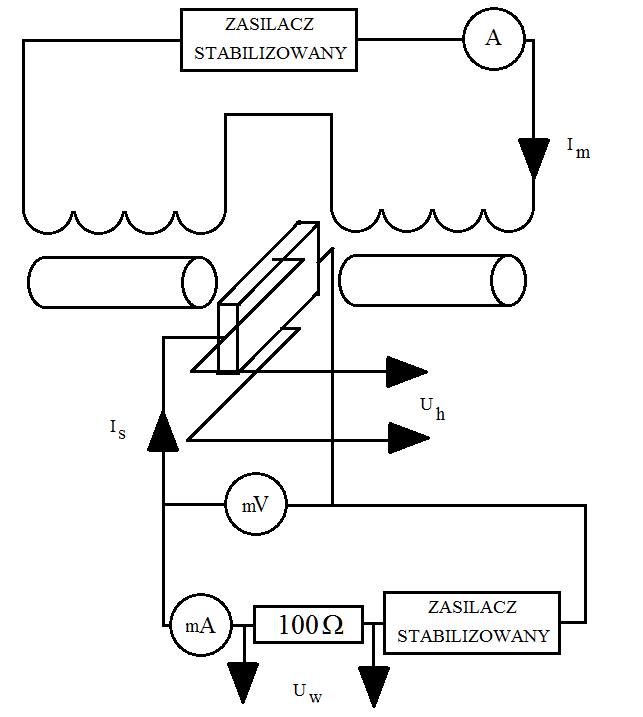
\includegraphics[width=10cm]{schemat.png}
\section{Prezentacja wyników pomiarów}
\hfill
\begin{tabular}{c|c|c|c|c|c|c|c|c}
N	&	$U_H [V]$	&	$u(U_H)$	&	$U[V]$	&	$u(U)$	&	 $I_s[mA]$	&	$u(I_s)$	&	 $U_{100\Omega}[V]$	&	$u(U_{100\Omega})$	 \\\hline
1	&	0,0010	&	0,0010	&	0,0158	&	0,0012	&	0,0400	&	0,0015	&		&		\\
2	&	0,0075	&	0,0011	&	0,1229	&	0,0025	&	0,3200	&	0,0048	&		&		\\
3	&	0,0141	&	0,0012	&	0,2310	&	0,0038	&	0,6100	&	0,0083	&		&		\\
4	&	0,0176	&	0,0012	&	0,2860	&	0,0044	&	0,7600	&	0,0101	&		&		\\
5	&	0,0227	&	0,0013	&	0,3690	&	0,0054	&	0,9800	&	0,0128	&		&		\\
6	&	0,0279	&	0,0013	&	0,4560	&	0,0065	&	1,2100	&	0,0155	&		&		\\
7	&	0,0325	&	0,0014	&	0,5300	&	0,0074	&	1,4100	&	0,0179	&		&		\\
8	&	0,0375	&	0,0015	&	0,6110	&	0,0083	&	1,6400	&	0,0207	&		&		\\
9	&	0,0423	&	0,0015	&	0,6910	&	0,0093	&	1,8600	&	0,0233	&		&		\\
10	&	0,0473	&	0,0016	&	0,7720	&	0,0103	&	2,0900	&	0,0261	&		&		\\
11	&	0,0520	&	0,0016	&	0,8490	&	0,0112	&	2,3100	&	0,0287	&		&		\\
12	&	0,0567	&	0,0017	&	0,9260	&	0,0121	&	2,5300	&	0,0314	&		&		\\
13	&	0,0612	&	0,0017	&	1,0000	&	0,0130	&	2,7500	&	0,0340	&		&		\\
14	&	0,0659	&	0,0018	&	1,0700	&	0,0138	&	2,9800	&	0,0368	&		&		\\
15	&	0,0703	&	0,0018	&	1,1400	&	0,0147	&	3,2000	&	0,0394	&	0,3130	&	0,0048	\\
16	&	0,0745	&	0,0019	&	1,2100	&	0,0155	&	3,4200	&	0,0420	&		&		\\
17	&	0,0790	&	0,0019	&	1,2900	&	0,0165	&	3,6500	&	0,0448	&		&		\\
18	&	0,0830	&	0,0020	&	1,3600	&	0,0173	&	3,8700	&	0,0474	&		&		\\
19	&	0,0870	&	0,0020	&	1,4200	&	0,0180	&	4,0900	&	0,0501	&		&		\\
20	&	0,0909	&	0,0021	&	1,4800	&	0,0188	&	4,3100	&	0,0527	&		&		\\
21	&	0,0946	&	0,0021	&	1,5500	&	0,0196	&	4,5300	&	0,0554	&		&		\\
22	&	0,0986	&	0,0022	&	1,6100	&	0,0203	&	4,7600	&	0,0581	&		&		\\
23	&	0,1021	&	0,0022	&	1,6700	&	0,0210	&	4,9800	&	0,0608	&		&		\\
24	&	0,1056	&	0,0023	&	1,7300	&	0,0218	&	5,2100	&	0,0635	&		&		\\
25	&	0,1090	&	0,0023	&	1,7900	&	0,0225	&	5,4300	&	0,0662	&		&		\\
26	&	0,1123	&	0,0023	&	1,8400	&	0,0231	&	5,6600	&	0,0689	&		&		\\
27	&	0,1155	&	0,0024	&	1,9000	&	0,0238	&	5,8800	&	0,0716	&		&		\\
28	&	0,1185	&	0,0024	&	1,9500	&	0,0244	&	6,1100	&	0,0743	&		&		\\
29	&	0,1216	&	0,0025	&	2,0000	&	0,0250	&	6,3300	&	0,0770	&		&		\\
30	&	0,1246	&	0,0025	&	2,0500	&	0,0256	&	6,5600	&	0,0797	&		&		\\

\end{tabular}
\captionof{table}{Dla $I = 0,1A$, $B = 0,0125T$}

\hfill
\begin{tabular}{c|c|c|c|c|c|c|c|c}
N	&	$U_H [V]$	&	$u(U_H)$	&	$U[V]$	&	$u(U)$	&	 $I_s[mA]$	&	$u(I_s)$	&	 $U_{100\Omega}[V]$	&	$u(U_{100\Omega})$	 \\\hline
1	&	0,0023	&	0,0010	&	0,0160	&	0,0012	&	0,0400	&	0,0015	&		&		 \\
2	&	0,0181	&	0,0012	&	0,1230	&	0,0025	&	0,3150	&	0,0048	&		&		 \\
3	&	0,0348	&	0,0014	&	0,2380	&	0,0039	&	0,6130	&	0,0084	&		&		 \\
4	&	0,0435	&	0,0015	&	0,2980	&	0,0046	&	0,7680	&	0,0102	&		&		 \\
5	&	0,0553	&	0,0017	&	0,3770	&	0,0055	&	0,9750	&	0,0127	&		&		 \\
6	&	0,0680	&	0,0018	&	0,4660	&	0,0066	&	1,2080	&	0,0155	&		&		 \\
7	&	0,0796	&	0,0020	&	0,5460	&	0,0076	&	1,4180	&	0,0180	&		&		 \\
8	&	0,0922	&	0,0021	&	0,6310	&	0,0086	&	1,6450	&	0,0207	&		&		 \\
9	&	0,1037	&	0,0022	&	0,7100	&	0,0095	&	1,8590	&	0,0233	&		&		 \\
10	&	0,1156	&	0,0024	&	0,7930	&	0,0105	&	2,0900	&	0,0261	&		&		 \\
11	&	0,1270	&	0,0025	&	0,8720	&	0,0115	&	2,3100	&	0,0287	&		&		 \\
12	&	0,1386	&	0,0027	&	0,9510	&	0,0124	&	2,5300	&	0,0314	&		&		 \\
13	&	0,1496	&	0,0028	&	1,0280	&	0,0133	&	2,7500	&	0,0340	&		&		 \\
14	&	0,1610	&	0,0029	&	1,1080	&	0,0143	&	2,9800	&	0,0368	&		&		 \\
15	&	0,1714	&	0,0031	&	1,1800	&	0,0152	&	3,2000	&	0,0394	&	0,3140	&	0,0048	 \\
16	&	0,1816	&	0,0032	&	1,2490	&	0,0160	&	3,4200	&	0,0420	&		&		 \\
17	&	0,1922	&	0,0033	&	1,3250	&	0,0169	&	3,6500	&	0,0448	&		&		 \\
18	&	0,2010	&	0,0034	&	1,3910	&	0,0177	&	3,8600	&	0,0473	&		&		 \\
19	&	0,2120	&	0,0035	&	1,4650	&	0,0186	&	4,1000	&	0,0502	&		&		 \\
20	&	0,2220	&	0,0037	&	1,5310	&	0,0194	&	4,3200	&	0,0528	&		&		 \\
21	&	0,2300	&	0,0038	&	1,5900	&	0,0201	&	4,5400	&	0,0555	&		&		 \\
22	&	0,2390	&	0,0039	&	1,6530	&	0,0208	&	4,7600	&	0,0581	&		&		 \\
23	&	0,2470	&	0,0040	&	1,7180	&	0,0216	&	4,9900	&	0,0609	&		&		 \\
24	&	0,2550	&	0,0041	&	1,7740	&	0,0223	&	5,2000	&	0,0634	&		&		 \\
25	&	0,2650	&	0,0042	&	1,8400	&	0,0231	&	5,4400	&	0,0663	&		&		 \\
26	&	0,2710	&	0,0043	&	1,8890	&	0,0237	&	5,6500	&	0,0688	&		&		 \\
27	&	0,2810	&	0,0044	&	1,9450	&	0,0243	&	5,8800	&	0,0716	&		&		 \\
28	&	0,2880	&	0,0045	&	2,0000	&	0,0250	&	6,1100	&	0,0743	&		&		 \\
29	&	0,2960	&	0,0046	&	2,0500	&	0,0256	&	6,3400	&	0,0771	&		&		 \\
30	&	0,3020	&	0,0046	&	2,1000	&	0,0262	&	6,5500	&	0,0796	&		&		 \\

\end{tabular}
\captionof{table}{Dla $I = 0,2A$, $B =0,025T $}

\hfill
\begin{tabular}{c|c|c|c|c|c|c|c|c}
N	&	$U_H [V]$	&	$u(U_H)$	&	$U[V]$	&	$u(U)$	&	 $I_s[mA]$	&	$u(I_s)$	&	 $U_{100\Omega}[V]$	&	$u(U_{100\Omega})$	 \\\hline
1	&	0,0037	&	0,0010	&	0,0179	&	0,0012	&	0,0440	&	0,0015	&		&		 \\
2	&	0,0281	&	0,0013	&	0,1345	&	0,0026	&	0,3320	&	0,0050	&		&		 \\
3	&	0,0517	&	0,0016	&	0,2460	&	0,0040	&	0,6100	&	0,0083	&		&		 \\
4	&	0,0650	&	0,0018	&	0,3050	&	0,0047	&	0,7560	&	0,0101	&		&		 \\
5	&	0,0828	&	0,0020	&	0,3930	&	0,0057	&	0,9770	&	0,0127	&		&		 \\
6	&	0,1017	&	0,0022	&	0,4840	&	0,0068	&	1,2050	&	0,0155	&		&		 \\
7	&	0,1193	&	0,0024	&	0,5680	&	0,0078	&	1,4200	&	0,0180	&		&		 \\
8	&	0,1370	&	0,0026	&	0,6520	&	0,0088	&	1,6420	&	0,0207	&		&		 \\
9	&	0,1548	&	0,0029	&	0,7400	&	0,0099	&	1,8640	&	0,0234	&		&		 \\
10	&	0,1734	&	0,0031	&	0,8280	&	0,0109	&	2,1000	&	0,0262	&		&		 \\
11	&	0,1898	&	0,0033	&	0,9050	&	0,0119	&	2,3000	&	0,0286	&		&		 \\
12	&	0,2070	&	0,0035	&	0,9890	&	0,0129	&	2,5300	&	0,0314	&		&		 \\
13	&	0,2240	&	0,0037	&	1,0680	&	0,0138	&	2,7500	&	0,0340	&		&		 \\
14	&	0,2410	&	0,0039	&	1,1470	&	0,0148	&	2,9800	&	0,0368	&		&		 \\
15	&	0,2560	&	0,0041	&	1,2230	&	0,0157	&	3,1900	&	0,0393	&	0,3130	&	0,0048	\\
16	&	0,2710	&	0,0043	&	1,2990	&	0,0166	&	3,4300	&	0,0422	&		&		 \\
17	&	0,2870	&	0,0044	&	1,3690	&	0,0174	&	3,6400	&	0,0447	&		&		 \\
18	&	0,3020	&	0,0046	&	1,4450	&	0,0183	&	3,8700	&	0,0474	&		&		 \\
19	&	0,3170	&	0,0048	&	1,5130	&	0,0192	&	4,0800	&	0,0500	&		&		 \\
20	&	0,3310	&	0,0050	&	1,5830	&	0,0200	&	4,3200	&	0,0528	&		&		 \\
21	&	0,3440	&	0,0051	&	1,6480	&	0,0208	&	4,5400	&	0,0555	&		&		 \\
22	&	0,3570	&	0,0053	&	1,7170	&	0,0216	&	4,7700	&	0,0582	&		&		 \\
23	&	0,3700	&	0,0054	&	1,7750	&	0,0223	&	4,9700	&	0,0606	&		&		 \\
24	&	0,3830	&	0,0056	&	1,8350	&	0,0230	&	5,2000	&	0,0634	&		&		 \\
25	&	0,3960	&	0,0058	&	1,8990	&	0,0238	&	5,4300	&	0,0662	&		&		 \\
26	&	0,4080	&	0,0059	&	1,9570	&	0,0245	&	5,6600	&	0,0689	&		&		 \\
27	&	0,4180	&	0,0060	&	2,0100	&	0,0251	&	5,8900	&	0,0717	&		&		 \\
28	&	0,4290	&	0,0061	&	2,0600	&	0,0257	&	6,1100	&	0,0743	&		&		 \\
29	&	0,4390	&	0,0063	&	2,1200	&	0,0264	&	6,3400	&	0,0771	&		&		 \\
30	&	0,4500	&	0,0064	&	2,1700	&	0,0270	&	6,5700	&	0,0798	&		&		 \\
\end{tabular}
\captionof{table}{Dla $I = 0,3A$, $B = 0,04T$}

\hfill
\begin{tabular}{c|c|c|c|c|c|c|c|c}
N	&	$U_H [V]$	&	$u(U_H)$	&	$U[V]$	&	$u(U)$	&	 $I_s[mA]$	&	$u(I_s)$	&	 $U_{100\Omega}[V]$	&	$u(U_{100\Omega})$	 \\\hline
1	&	0,0048	&	0,0011	&	0,0178	&	0,0012	&	0,0420	&	0,0015	&		&		 \\
2	&	0,0385	&	0,0015	&	0,1435	&	0,0027	&	0,3360	&	0,0050	&		&		 \\
3	&	0,0697	&	0,0018	&	0,2600	&	0,0041	&	0,6100	&	0,0083	&		&		 \\
4	&	0,0863	&	0,0020	&	0,3210	&	0,0049	&	0,7560	&	0,0101	&		&		 \\
5	&	0,1109	&	0,0023	&	0,4130	&	0,0060	&	0,9750	&	0,0127	&		&		 \\
6	&	0,1358	&	0,0026	&	0,5060	&	0,0071	&	1,1980	&	0,0154	&		&		 \\
7	&	0,1632	&	0,0030	&	0,5980	&	0,0082	&	1,4190	&	0,0180	&		&		 \\
8	&	0,1857	&	0,0032	&	0,6930	&	0,0093	&	1,6510	&	0,0208	&		&		 \\
9	&	0,2080	&	0,0035	&	0,7770	&	0,0103	&	1,8610	&	0,0233	&		&		 \\
10	&	0,2320	&	0,0038	&	0,8650	&	0,0114	&	2,0800	&	0,0260	&		&		 \\
11	&	0,2570	&	0,0041	&	0,9580	&	0,0125	&	2,3200	&	0,0288	&		&		 \\
12	&	0,2780	&	0,0043	&	1,0380	&	0,0135	&	2,5300	&	0,0314	&		&		 \\
13	&	0,3000	&	0,0046	&	1,1200	&	0,0144	&	2,7400	&	0,0339	&		&		 \\
14	&	0,3220	&	0,0049	&	1,2030	&	0,0154	&	2,9700	&	0,0366	&		&		 \\
15	&	0,3440	&	0,0051	&	1,2850	&	0,0164	&	3,2000	&	0,0394	&	0,3140	&	0,0048	\\
16	&	0,3640	&	0,0054	&	1,3620	&	0,0173	&	3,4200	&	0,0420	&		&		 \\
17	&	0,3850	&	0,0056	&	1,4380	&	0,0183	&	3,6400	&	0,0447	&		&		 \\
18	&	0,4040	&	0,0058	&	1,5110	&	0,0191	&	3,8600	&	0,0473	&		&		 \\
19	&	0,4240	&	0,0061	&	1,5860	&	0,0200	&	4,0900	&	0,0501	&		&		 \\
20	&	0,4460	&	0,0064	&	1,6570	&	0,0209	&	4,3100	&	0,0527	&		&		 \\
21	&	0,4620	&	0,0065	&	1,7260	&	0,0217	&	4,5300	&	0,0554	&		&		 \\
22	&	0,4800	&	0,0068	&	1,7960	&	0,0226	&	4,7600	&	0,0581	&		&		 \\
23	&	0,4960	&	0,0070	&	1,8580	&	0,0233	&	4,9700	&	0,0606	&		&		 \\
24	&	0,5130	&	0,0072	&	1,9240	&	0,0241	&	5,2100	&	0,0635	&		&		 \\
25	&	0,5280	&	0,0073	&	1,9810	&	0,0248	&	5,4200	&	0,0660	&		&		 \\
26	&	0,5440	&	0,0075	&	2,0400	&	0,0255	&	5,6500	&	0,0688	&		&		 \\
27	&	0,5580	&	0,0077	&	2,1000	&	0,0262	&	5,8800	&	0,0716	&		&		 \\
28	&	0,5740	&	0,0079	&	2,1500	&	0,0268	&	6,1000	&	0,0742	&		&		 \\
29	&	0,5870	&	0,0080	&	2,2100	&	0,0275	&	6,3200	&	0,0768	&		&		 \\
30	&	0,6000	&	0,0082	&	2,2600	&	0,0281	&	6,5500	&	0,0796	&		&		 \\
\end{tabular}
\captionof{table}{Dla $I = 0,4A$, $B = 0,05T$}

\newpage
\section{Obliczenia i wykresy}
Obliczeń dokonaliśmy metodą najmniejszych kwadratów. Wykresy sporządzone za pomocą tych obliczeń znajdują się poniżej. Niepewność miernika liczyliśmy według wzoru
\begin{equation}
1,2\% \cdot \text{ wartość } + 0,001 [V]
\end{equation} 
$R_h$ liczyliśmy dwoma sposobami: z proporcji
\begin{equation}
R_h = \frac{U\cdot 100\Omega}{U_{w 100\Omega}}
\end{equation} 
i ze wzoru ~\ref{fig:rhwzor}. Wartości policzone dwoma sposobami dla każdego podpunktu są do siebie zbliżone.

%Korzystając ze wzorów ~\ref{fig:nwzor} i ~\ref{fig:muwzor} oraz obliczając niepewność standardową za pomocą wzorów ~\ref{fig:niep1} i ~\ref{fig:niep2}

%Wykresy sporządzone na podstawie wyników powyższych obliczeń. Niepewność miernika liczona według wzoru $1,2\% \cdot \text{ wartość } + 0,001 [V] $
\subsection{$I_m=0,1 \Rightarrow B=0,0125$}
\begin{equation}
n = \frac{51,997 \cdot 10^{-3} \cdot 0,0125T }{ 0,2\mu m \cdot 1,602 \cdot 10^{-19}C} = 2,029(0,032)\cdot10^{22} [\mu^{-1}]
\end{equation} 
\begin{equation}
\mu = \frac{0,0609\cdot0,1A }{40\cdot10^{-6}m \cdot 0,0125T} = 12180(19)\frac{A}{mT}
\end{equation} 
Z proporcji
\begin{equation}
R_h = \frac{1,14V * 100\Omega}{0,313V} = 364,22(3,38)\Omega
\end{equation} 
\begin{equation}
R_h = \frac{l}{ne\mu cd}
\end{equation} 
\begin{equation}
R_h = \frac{0,1}{2,029\cdot 10^{22} \cdot 1,602\cdot10^{-19} \cdot 12180 \cdot 40 \cdot 0,2 \cdot 10^{-12}} = 315,73(2,96) \Omega
\end{equation} 
\begin{equation}
	u(R_H) = \sqrt{\left(\frac{\delta f(n,\mu)}{\delta n}\right)^2 u^2(n) + \left(\frac{\delta f(n,\mu)}{\delta\mu}\right)^2 u^2(\mu)}
\end{equation}
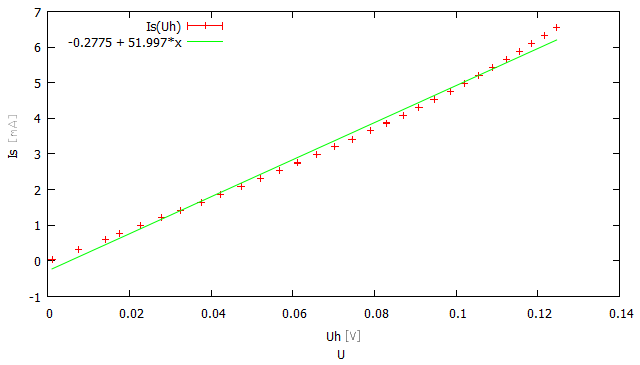
\includegraphics[width=10cm]{21.png}
\captionof{figure}{Wykres $U_H(I_S)$ dla $I_m=0,1 $}
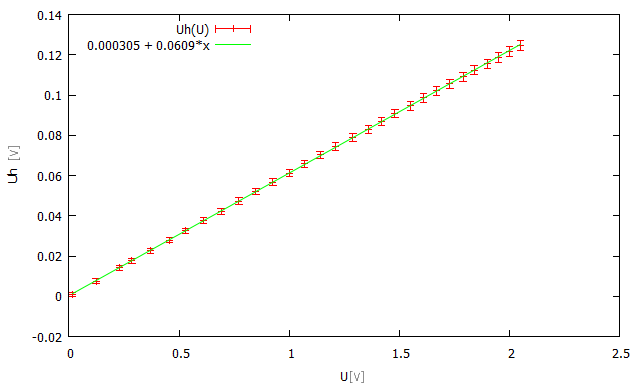
\includegraphics[width=10cm]{11.png}
\captionof{figure}{Wykres $U_H(U)$ dla $I_m=0,1 $}


% 2 
\subsection{$I_m=0,2 \Rightarrow B=0,025$}
\begin{equation}
n = 1,675(0,027)\cdot 10^{22}[\mu^{-1}]
\end{equation} 
\begin{equation}
\mu = 28720(42)\frac{A}{mT}
\end{equation} 
Z proporcji:
\begin{equation}
R_h = 375,80(3,52)\Omega
\end{equation} 
\begin{equation}
R_h = 324,3981(3,06)\Omega
\end{equation} 

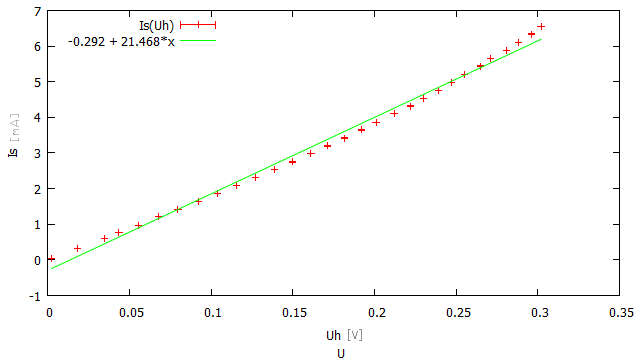
\includegraphics[width=10cm]{22.png}
\captionof{figure}{Wykres $U_H(I_S)$ dla $I_m=0,2 $}
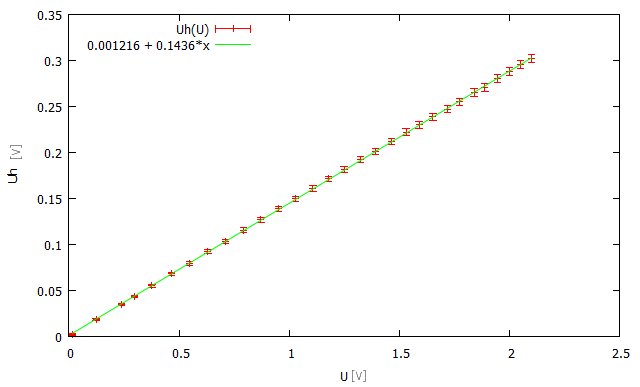
\includegraphics[width=10cm]{12.png}
\captionof{figure}{Wykres $U_H(U)$ dla $I_m=0,2 $}

% 3
\subsection{$I_m=0,3 \Rightarrow B=0,04T$}
\begin{equation}
n = 1,796(0,023)\cdot 10^{22}[\mu^{-1}]
\end{equation} 
\begin{equation}
\mu = 38925(51)\frac{A}{mT}
\end{equation} 
Z proporcji:
\begin{equation}
R_h = 390,73(3,66)\Omega
\end{equation} 
\begin{equation}
R_h = 334,8373(3,12)\Omega
\end{equation} 

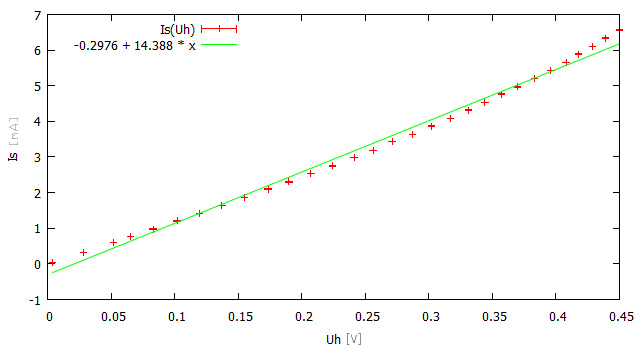
\includegraphics[width=10cm]{23.png}
\captionof{figure}{Wykres $U_H(I_S)$ dla $I_m=0,3 $}
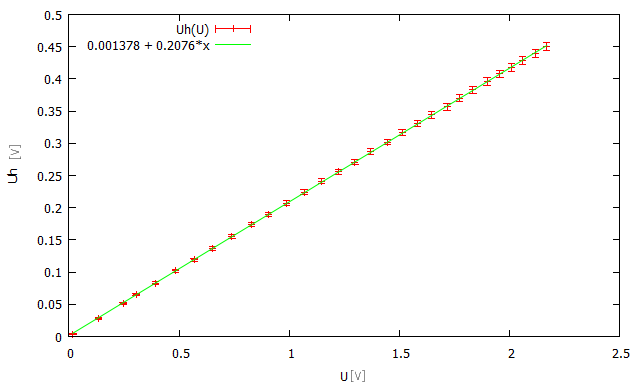
\includegraphics[width=10cm]{13.png}
\captionof{figure}{Wykres $U_H(U)$ dla $I_m=0,3 $}

% 4
\subsection{$I_m=0,4 \Rightarrow B=0,05$}
\begin{equation}
n = 1,678(0,024)\cdot 10^{22}[\mu^{-1}]
\end{equation} 
\begin{equation}
\mu = 53194(73)\frac{A}{mT}
\end{equation} 
Z proporcji:
\begin{equation}
R_h = 409,24(4,02)\Omega
\end{equation} 
\begin{equation}
R_h = 349,6656(3,21)\Omega
\end{equation} 

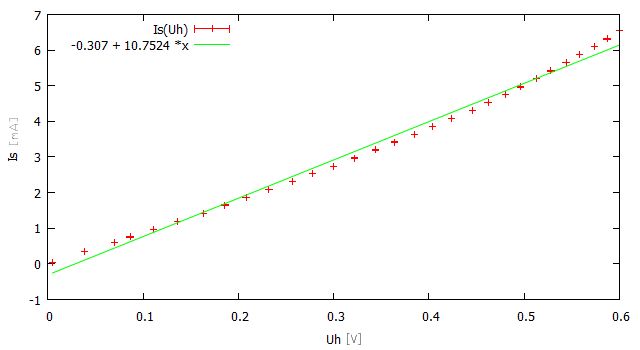
\includegraphics[width=10cm]{24.png}
\captionof{figure}{Wykres $U_H(I_S)$ dla $I_m=0,4 $}
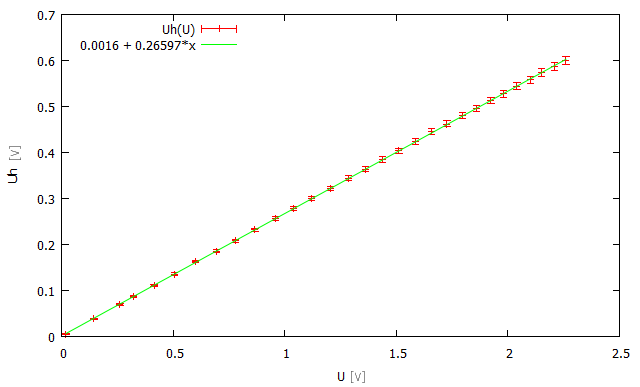
\includegraphics[width=10cm]{14.png}
\captionof{figure}{Wykres $U_H(U)$ dla $I_m=0,4 $}

\section{Wnioski}

W ćwiczeniu zapoznaliśmy się ze zjawiskiem efektu Halla. Zgodnie z przewidywaniami teoretycznymi, napięcie Halla $U_H$ w naszych pomiarach jest proporcjonalne do wielkości indukcji magnetycznej oraz natężenia prądu sterującego.\\

Wyznaczona przez nas koncentracja elektronów swobodnych $n = wstawic $ daje nam możliwość ustalenia właściwości elektrycznych metalu, z którego wykonana została płytka hallotronu. Zajęcia laboratoryjne dały nam odpowiedź na pytnie o powód tak szerokiego zastosowania hallotronu w praktyce.\\

Przeprowadzone ćwiczenia potwierdziły liniowość zależności \underline{(wykresy niemalże liniowe)}, a więc zgodność z założeniami teoretycznymi.

\end{document}
 
